\documentclass[12pt]{amsart}
\usepackage{amssymb}
\usepackage{cite}
\usepackage{array}
\usepackage{booktabs}
\usepackage{mdwtab}
\usepackage{mathtools}
\usepackage[T1]{fontenc}
\usepackage[utf8]{inputenc}
\usepackage{hyphenat}
\usepackage{enumitem}
\usepackage{ifpdf}
\ifpdf
  \usepackage[pdftex]{graphicx}
  \usepackage[pdftex,margin=1.25in]{geometry}
  \usepackage[bookmarks=true, bookmarksopen=true,%
    bookmarksdepth=3,bookmarksopenlevel=2,%
    colorlinks=true,%
    linkcolor=blue,%
    citecolor=blue,%
    filecolor=blue,%
    menucolor=blue,%
    urlcolor=blue]{hyperref}
  \hypersetup{pdftitle={Towards the quantum exceptional series}}
  \hypersetup{pdfauthor={Scott Morrison, Noah Snyder, and Dylan P. Thurston}}
\else
  \usepackage[dvips]{graphicx}
  \usepackage[dvips,margin=1in]{geometry}
  % Use hyperref with all features turned off even in DVI mode, since
  % the .aux file format changes
  \usepackage[draft]{hyperref}
\fi
\usepackage{url}
\usepackage{todonotes}

% A binary operator with a subscript on both sides (and correct spacing)
% Name stands for subscript-operator-subscript
\newcommand{\sos}[3]{\mathbin{{}_{#1}\mathord#2_{#3}}}

% manyindices
% Adapted from code by "bza" in comp.text.tex, Feb. 7, 2006
%% USAGE:
%%
%% \manyindices#1#2#3#4#5
%%
%% #1=lower left index
%% #2=upper left index
%% #3=lower right index
%% #4=upper right index
%% #5=main symbol
\makeatletter
\newcommand\mi@kern[1]{%
  \settowidth\@tempdima{$\mi@obj^{#1}$}
  \kern-\@tempdima
  #1
  \settowidth\@tempdima{$\mi@obj$}
  \kern\@tempdima
}

\newtoks\mi@toksp
\newtoks\mi@toksb
\DeclareRobustCommand{\manyindices}[5]{
  \def\mi@obj{#5}
  \mi@toksp\expandafter{\mi@kern{#2}}
  \mi@toksb\expandafter{\mi@kern{#1}}
  \@mathmeasure4\textstyle{#5_{#1}^{#2}}
  \@mathmeasure6\textstyle{#5_{#3}^{#4}}
  \dimen0-\wd6 \advance\dimen0\wd4
  \@mathmeasure8\textstyle{\hphantom{{}_{#1}^{#2}}#5^{\the\mi@toksp#4}_{\the\mi@toksb#3}}
  \hbox to \dimen0{}{\kern-\dimen0\box8}
}
\makeatother 

% Left sub/super scripts
% \lsup is a temporary definition until something better is worked out
% Use \lsupv if the next argument is vertical
\newcommand{\lsub}[2]{{}_{#1}#2}
\newcommand{\lsup}[2]{{}^{#1}\mskip-.6\thinmuskip#2}
\newcommand{\lsupv}[2]{{}^{#1}#2}
\newcommand{\lsubsup}[3]{\manyindices{#1}{\mskip.6\thinmuskip#2\mskip-.6\thinmuskip}{}{}{\mathord{#3}}}
\newcommand{\lsubsupv}[3]{\manyindices{#1}{\mskip.2\thinmuskip#2\mskip-.2\thinmuskip}{}{}{\mathord{#3}}}

\newcounter{saveenum}

% Read the file, if it exists
\newread\testin
\def\maybeinput#1{
\openin\testin=#1
\ifeof\testin\typeout{Warning: input #1 not found}\else\input#1\fi
\closein\testin
}

\def\mathcenter#1{%
  \vcenter{\hbox{$#1$}}%
}

\def\graph#1{
        \includegraphics{#1}
}

\def\mathgraph#1{
        \mathcenter{\graph{#1}}
}

\def\mfig#1{
        \mathcenter{\includegraphics{#1}}
}

\def\mfigb#1{
        \mathcenter{\includegraphics[trim=-1 -1 -1 -1]{#1}}
}


%%% Local Variables: 
%%% mode: latex
%%% TeX-master: "main"
%%% End: 

% General use
\newcommand{\RR}{\mathbb R}
\newcommand{\CC}{\mathbb C}
\newcommand{\ZZ}{\mathbb Z}
\newcommand{\QQ}{\mathbb Q}
\newcommand{\PP}{\mathbb P}
\newcommand{\EE}{\mathbb E}
\newcommand{\HH}{\mathbb H}
\newcommand{\NN}{\mathbb N}

\newcommand{\comma}{\mathbin ,}
\newcommand{\conn}{\mathbin \#}
\newcommand{\sltwo}{{{\mathfrak{sl}}_2}}
\renewcommand{\sl}{\mathfrak{sl}}
\newcommand{\gl}{\mathfrak{gl}}
\newcommand{\fg}{{\mathfrak g}}
\newcommand{\co}{\colon\thinspace}
\newcommand{\eps}{\varepsilon}
\newcommand{\abs}[1]{{\lvert #1 \rvert}}
\newcommand{\norm}[1]{{\lVert #1 \rVert}}
\newcommand{\OneHalf}{{\textstyle\frac{1}{2}}}

% Synonyms for commands I never remember
\newcommand{\isom}{\cong}
\newcommand{\superset}{\supset}
\newcommand{\bigcircle}{\bigcirc}
\newcommand{\contains}{\ni}
\newcommand{\tensor}{\otimes}
\newcommand{\bdy}{\partial}

% Stupid overloading.
\newcommand{\lbracket}{[}
\newcommand{\rbracket}{]}

% Various operators.
\DeclareMathOperator{\ad}{ad}
\DeclareMathOperator{\Ad}{Ad}
\DeclareMathOperator{\End}{End}
\DeclareMathOperator{\sign}{sign}
\DeclareMathOperator{\Sym}{Sym}
\DeclareMathOperator{\tr}{tr}
\DeclareMathOperator{\Hom}{Hom}
\DeclareMathOperator{\vol}{vol}
\DeclareMathOperator{\rank}{rank}
\DeclareMathOperator{\im}{im}

% Linear groups
\DeclareMathOperator{\ISO}{\mathit{ISO}}
\DeclareMathOperator{\SO}{\mathit{SO}}
\DeclareMathOperator{\GL}{\mathit{GL}}
\DeclareMathOperator{\SL}{\mathit{SL}}
\DeclareMathOperator{\PSL}{\mathit{PSL}}

% citations
\newcommand{\arxiv}[1]{\href{http://arxiv.org/abs/#1}{\tt arXiv:\nolinkurl{#1}}}
\newcommand{\doi}[1]{\href{http://dx.doi.org/#1}{{\tt DOI:#1}}}
\newcommand{\euclid}[1]{\href{http://projecteuclid.org/getRecord?id=#1}{{\tt #1}}}
\newcommand{\mathscinet}[1]{\href{http://www.ams.org/mathscinet-getitem?mr=#1}{\tt #1}}
\newcommand{\googlebooks}[1]{(preview at \href{http://books.google.com/books?id=#1}{google books})}
\renewcommand{\googlebooks}[1]{}
\newcommand{\numdam}[1]{\href{http://www.numdam.org/item?id=#1}{\tt #1}}

% Theorems
\theoremstyle{plain}
\newtheorem{theorem}{Theorem}
\newtheorem{proposition}{Proposition}
\numberwithin{proposition}{section}
\newtheorem{lemma}[proposition]{Lemma}
\newtheorem{corollary}[proposition]{Corollary}
\newtheorem{claim}[proposition]{Claim}
\newtheorem{conjecture}[proposition]{Conjecture}
\newtheorem{observation}[proposition]{Observation}

\theoremstyle{definition}
\newtheorem{definition}[proposition]{Definition}
\newtheorem{exercise}[proposition]{Exercise}
\newtheorem{question}[proposition]{Question}
\newtheorem{problem}[proposition]{Problem}

\theoremstyle{remark}
\newtheorem{example}[proposition]{Example}
%\newtheorem{hint}[proposition]{Hint}
\newtheorem{remark}[proposition]{Remark}
%\newtheorem{apology}[proposition]{Apology}
%\newtheorem{warning}[proposition]{Warning}

% Hyphenation.
\hyphenation{Thurs-ton}

%ToDoNotes:
\newcommand{\nn}[1]{{\color{red}[[#1]]}}
\newcommand{\DPTtodo}[1]{\todo[color=green!40]{#1}}
\newcommand{\NStodo}[1]{\todo[color=blue!40]{#1}}
\newcommand{\SMtodo}[1]{\todo[color=red!40]{#1}}
\newcommand{\citationneeded}{\ \parbox{1.25in}{\todo[inline]{citation needed}}\ }
\newcommand{\referenceneeded}{\ \parbox{1.35in}{\todo[inline]{reference needed}}\ }

% Commands for exceptional paper
\newcommand{\Sk}[1]{\mathop{\mathrm{Sk}}(#1)}
\newcommand{\Skq}[1]{\mathop{\mathrm{Sk}_q}(#1)}
\newcommand{\Skcat}{\mathop{\mathsf{Sk}}}
\newcommand{\Skqcat}{\mathop{\mathsf{Sk}_q}}
\DeclareMathOperator{\eval}{eval}

\DeclareMathOperator{\Tw}{Tw}
\DeclareMathOperator{\HTw}{HTw}
\DeclareMathOperator{\Fr}{Fr}

\DeclareMathOperator{\fork}{fork}
\DeclareMathOperator{\fuse}{fuse}


%%% Local Variables: 
%%% mode: latex
%%% TeX-master: "main"
%%% TeX-master: t
%%% End: 

\usepackage{fp}
\usepackage{tikz}
\usetikzlibrary{matrix}
\usetikzlibrary{arrows,backgrounds,patterns,scopes,external,hobby,
    decorations.pathreplacing,
    decorations.pathmorphing
}

\newlength{\fuzzwidth}
\setlength{\fuzzwidth}{2.5pt}
\newlength{\arrowlength}
\setlength{\arrowlength}{8pt}
\newlength{\arrowwidth}
\setlength{\arrowwidth}{.75pt}
\newlength{\pointrad}
\setlength{\pointrad}{1.5pt}
\newlength{\linewid}
\setlength{\linewid}{1.5pt}
\newlength{\circlerad}
\setlength{\circlerad}{16pt}
\newlength{\smcirclerad}
\setlength{\smcirclerad}{8pt}
\newcommand{\fillcolor}{black!60}
\newcommand{\fuzzcolor}{black!25}
\newcommand{\arrowcolor}{black!25}
\newcommand{\covercolor}{black!0}
\newcommand{\graycolor}{black!55}
\newcommand{\graylightcolor}{black!40}


\newcommand{\coverwidthfuzz}{6pt}
\newcommand{\coverwidth}{3.5pt}
\newcommand{\coverwidththin}{3.25pt}
\newcommand{\coverwidththick}{3.75pt}

\newlength{\linewidthin}
\setlength{\linewidthin}{1.25pt}
\newlength{\linewidthick}
\setlength{\linewidthick}{1.75pt}


\tikzset{use Hobby shortcut}
\tikzset{
	coverline/.style={
	preaction={draw,line width=\coverwidth,\covercolor}}, 
	coverlinethin/.style={
	preaction={draw,line width=\coverwidththin,\covercolor}}, 
	coverlinethick/.style={
	preaction={draw,line width=\coverwidththick,\covercolor}}, 
	coverlineleft/.style={
	preaction={draw,line width=\coverwidthfuzz,\covercolor,decorate,decoration={curveto,amplitude=0,raise=.35*\fuzzwidth}}}, %%% Notice this number was tweaked, 	
coverlinelefttail/.style={
	preaction={draw,line width=\coverwidthfuzz,\covercolor,decorate,decoration={curveto,amplitude=0,raise=.35*\fuzzwidth,pre=moveto,pre length=2pt}}}, %%% Notice this number was tweaked, probably will not look good if parameters change.  Again here, pre removes the raise option.
        fuzzlefttail/.style={
        preaction={draw,line width=\fuzzwidth,\fuzzcolor,decorate,decoration={curveto,pre=moveto,pre length=2pt,amplitude=0,raise=.5*\fuzzwidth}}}, %%% This does not work --- somehow pre breaks the raise function.
        linestylethin/.style={line width=\linewidthin},
        linestylethick/.style={line width=\linewidthick},
        linestylegray/.style={line width=\linewid,\graycolor},
        linestylegraylight/.style={line width=\linewid,\graylightcolor}
}
\tikzset{
        fuzzright/.style={
        preaction={draw,line width=\fuzzwidth,\fuzzcolor,decorate,decoration={curveto,amplitude=0,raise=-.5*\fuzzwidth}}},
        fuzzleft/.style={
        preaction={draw,line width=\fuzzwidth,\fuzzcolor,decorate,decoration={curveto,amplitude=0,raise=.5*\fuzzwidth}}},
        fuzzrightpre/.style={ %%% Doesn't work
        preaction={draw,line width=2pt,\fuzzcolor,decorate,decoration={curveto,amplitude=0,raise=-1pt,pre=moveto,pre length=12pt}}},
        fuzzleftpre/.style={ %%% Doesn't work
        preaction={draw,line width=2pt,\fuzzcolor,decorate,decoration={curveto,post=moveto,post length=32pt,amplitude=0,raise=1pt}}},        
        outstyle/.style={\arrowcolor, line width=\arrowwidth},
        linestyle/.style={line width=\linewid}
}

\newcommand{\lilarrow}{
\draw[->] (0,0) -- (1,0);
}

\newcommand{\cb}{\raisebox{.6ex-.5\height}}


%%%% These draw triple or quadruple set of arrows of length 0.5 cm
\DeclareMathOperator{\rightdoublearrows} {{\; 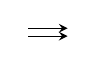
\begin{tikzpicture} \foreach \y in {0.05, 0.15} { \draw [-stealth] (0, \y) -- +(0.5, 0);} \; \end{tikzpicture}}}
\DeclareMathOperator{\leftdoublearrows} {{\; 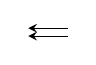
\begin{tikzpicture} \foreach \y in {0.05, 0.15} { \draw [stealth-] (0, \y) -- +(0.5, 0);} \; \end{tikzpicture}}}
\DeclareMathOperator{\righttriplearrows} {{\; 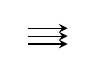
\begin{tikzpicture} \foreach \y in {0, 0.1, 0.2} { \draw [-stealth] (0, \y) -- +(0.5, 0);} \; \end{tikzpicture}}}
\DeclareMathOperator{\lefttriplearrows} {{\; 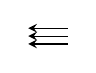
\begin{tikzpicture} \foreach \y in {0, 0.1, 0.2} { \draw [stealth-] (0, \y) -- +(0.5, 0);} \; \end{tikzpicture}}}
\DeclareMathOperator{\rightquadarrows} {{\; 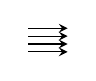
\begin{tikzpicture} \foreach \y in {-0.05, 0.05, 0.15, 0.25} { \draw [-stealth] (0, \y) -- +(0.5, 0);} \; \end{tikzpicture}}}
\DeclareMathOperator{\leftquadarrows} {{\; 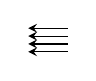
\begin{tikzpicture} \foreach \y in {-0.05, 0.05, 0.15, 0.25} { \draw [stealth-] (0, \y) -- +(0.5, 0);} \; \end{tikzpicture}}}

\newcommand{\ngon}[2][0]{
\begin{tikzpicture}[baseline=-0.5ex,scale=0.8]
\foreach \x in {1, ..., #2}
	\draw (360*\x/#2+#1:.8cm)--(360*\x/#2+#1:.5cm);
\foreach \x in {1, ..., #2}
	\draw (360*\x/#2+#1:.5cm) .. controls +(360*\x/#2+120+#1:.3cm) and +(360*\x/#2+360/#2-120+#1:.3cm) .. (360*\x/#2+360/#2+#1:.5cm);
\end{tikzpicture}
}

\newcommand{\nvertex}[2][0]{
\begin{tikzpicture}[baseline=-0.5ex,scale=0.8]
\foreach \x in {1, ..., #2}
	\draw (360*\x/#2+#1:.8cm)--(0,0);
\end{tikzpicture}
}

\newcommand{\unknot}{
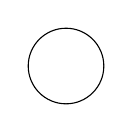
\begin{tikzpicture}[baseline=-0.5ex,scale=0.8]
  \draw (0,0) circle (.6cm);
\end{tikzpicture}
}

\newcommand{\drawI}{ 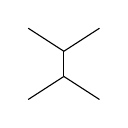
\begin{tikzpicture}[baseline=-0.5ex,scale=0.8]
 	\draw (0,.2) -- (45:.8cm);
 	\draw (0,.2) -- (135:.8cm);
	\draw (0,.2) -- (0,-.2);
 	\draw (0,-.2) -- (-45:.8cm);
 	\draw (0,-.2) -- (-135:.8cm);
\end{tikzpicture}
}

\newcommand{\drawH}{ 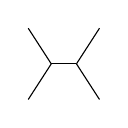
\begin{tikzpicture}[baseline=-0.5ex,rotate=90,scale=0.8]
 	\draw (0,.2) -- (45:.8cm);
 	\draw (0,.2) -- (135:.8cm);
	\draw (0,.2) -- (0,-.2);
 	\draw (0,-.2) -- (-45:.8cm);
 	\draw (0,-.2) -- (-135:.8cm);
\end{tikzpicture}}

\newcommand{\onestrandid}{\begin{tikzpicture}[baseline=-0.5ex,scale=0.8]
	\draw (-.8cm,0)--(.8cm,0);
\end{tikzpicture}}

\newcommand{\twostrandid}{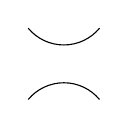
\begin{tikzpicture}[baseline=-0.5ex,scale=0.8]
	\draw (45:.8cm) to [curve through=(90:.3cm)] (135:.8cm);
	\draw (-45:.8cm) to [curve through=(-90:.3cm)] (-135:.8cm);
\end{tikzpicture}}

\newcommand{\cupcap}{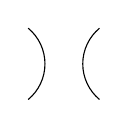
\begin{tikzpicture}[baseline=-0.5ex,rotate=90,scale=0.8]
	\draw (45:.8cm) to [curve through=(90:.3cm)] (135:.8cm);
	\draw (-45:.8cm) to [curve through=(-90:.3cm)] (-135:.8cm);
\end{tikzpicture}}

\newcommand{\symcross}{
\begin{tikzpicture}[baseline=-0.5ex,scale=0.8]
	\draw (45:.8cm) -- (-135:.8cm);
	\draw (-45:.8cm) -- (135:.8cm);
\end{tikzpicture}}

\newcommand{\braidcross}{
\begin{tikzpicture}[baseline=-0.5ex,scale=0.8]
	\draw (45:.8cm) -- (-135:.8cm);
	\draw[line width=1mm,white,double=black] (-45:.8cm) -- (135:.8cm);
\end{tikzpicture}}


\newcommand{\drawcrossX}{ 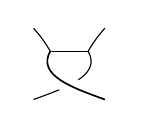
\begin{tikzpicture}[baseline=-0.5ex,scale=0.8,rotate=90]
 	\draw ([out angle=30].2,.3) .. (45:.8cm);
	\draw (.2,.3) -- (.2,-.3);
 	\draw ([out angle=-30].2,-.3) .. (-45:.8cm);
        \draw ([out angle=-150].2,-.3) ..([in angle=-70]135:.8cm);
 	\draw[line width=1mm,white,double=black]
              ([out angle=150].2,.3) .. ([in angle=70]-135:.8cm);
\end{tikzpicture}}

\newcommand{\twist}{
  
\begin{tikzpicture}[baseline=-0.5ex,scale=0.8]
    \draw[line width=1mm,white,double=black]
       ([out angle=-15]135:.8cm)..([blank=soft]-60:.4cm)..(-120:.4cm)..([in angle=-165]45:.8cm);
    \draw[line width=1mm,white,double=black,use previous Hobby path={invert soft blanks,disjoint}];
  \end{tikzpicture}}

\newcommand{\twistvertex}{
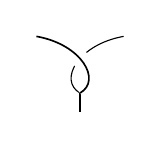
\begin{tikzpicture}[baseline=-0.5ex,scale=0.8]
  \draw (0,-0.5)--(0,-0.8);
  \draw ([out angle=-170]30:0.8cm)..([in angle=150](0,-0.5);
  \draw[line width=1mm,white,double=black]
        ([out angle=-10]150:0.8cm)..([in angle=30](0,-0.5);
\end{tikzpicture}}

\newcommand{\loopvertex}{

\begin{tikzpicture}[baseline=-0.5ex,scale=0.8]
  \draw (0,-0.5)--(0,-0.8);
  \draw ([out angle=150]0,-0.5)..(-0.02,0.6)..(0.02,0.6)..([in angle=30]0,-0.5);
\end{tikzpicture}
}

\newcommand{\pentagon}{
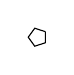
\begin{tikzpicture}[scale=.12,baseline=-2]
\draw (36:1) -- (108:1) -- (180:1) -- (252:1) -- (-36:1) -- (36:1);
\end{tikzpicture}
}

\newcommand{\psq}{
\begin{tikzpicture}[scale=.15,baseline=-2]
\draw (36:1) -- (108:1) -- (180:1) -- (252:1) -- (-36:1) -- (36:1) -- +(1.2,0) -- ($(-36:1)+(1.2,0)$) -- (-36:1);
\end{tikzpicture}
}

\newcommand{\sqsq}{
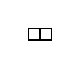
\begin{tikzpicture}[scale=.15]
\draw (0,0) -- (2,0) -- (2,1) -- (0,1) -- cycle (1,0) -- (1,1);
\end{tikzpicture}
}


\begin{document}
\title{Towards the quantum exceptional series}

\author[Morrison]{Scott Morrison}
\address{Mathematical Sciences Institute, Australian National University}
\email{scott.morrison@anu.edu.au}

\author[Snyder]{Noah Snyder}
\address{Bloomington, Indiana, USA}
\email{nsnyder1@indiana.edu} % Noah, do you prefer a different e-mail address?

\author[Thurston]{Dylan~P.~Thurston}
\address{Bloomington, Indiana, USA}
\email{dpthurst@indiana.edu}

\begin{abstract}
  We find a single two-parameter skein relation on trivalent graphs,
  the \emph{quantum exceptional relation}, that specializes to a skein
  relation associated to each exceptional Lie algebra (in the adjoint
  representation). If a slight
  strengthening of Deligne's conjecture on the existence of a
  (classical) exceptional series is true, then this relation
  holds for a new two-variable quantum exceptional polynomial, at
  least as a power series near $q=1$. The
  single quantum exceptional relation implies both the
  Jacobi relation (true for every Lie algebra) and
  the Vogel relation holding for the exceptional series.

  We find a conjectural basis for the space of diagrams with $n$ loose
  ends modulo the quantum exceptional relation for $n \le 7$, with
  dimensions agreeing with the classical computations, and compute
  the matrix of inner products. (Dimensions of idempotents?)
  We use the
  skein relation to compute the conjectural quantum exceptional
  polynomial for many knots, in particular
  determining unconditionally the values of the quantum polynomials
  for the exceptional Lie algebras in the adjoint representation on
  these knots.
\end{abstract}

%\subjclass[2000]{Primary xxx; Secondary xxx}
%\keywords{}

\maketitle

\tableofcontents

\section{Outline}
\label{sec:outline}

\begin{enumerate}
\item Introduction
  \begin{enumerate}
  \item Classical exceptional background
    \begin{enumerate}
    \item Jacobi and Vogel relations
    \item Reduction conjecture
    \item Consistency conjecture
    \item Something about the $n$-box space, or perhaps delay. (Could
      ask for finite-dimensionality, or positive-definite pairing
    \end{enumerate}
  \item Quantum exceptional results and conjectures
    \begin{enumerate}
    \item Skein relations
      \begin{enumerate}
      \item Framing change
      \item New relation (state uniqueness)
      \item Implies both classical relations in $q \to 1$ limit
      \item Mention other consequences, including double-crossing switch
      \end{enumerate}
    \item Conjectures: Reduction, consistency, $n$-box space
    \item Classical consistency $\Rightarrow$ quantum consistency.
    \end{enumerate}
  \item Dimensions of $n$-box spaces
  \item Evaluations we can compute easily
    \begin{enumerate}
    \item Exceptional computations hard previously
    \item With double-clasp switch
    \item Knots with width $\le$ 3
    \end{enumerate}
  \end{enumerate}
\item Background: More on classical conjectures, etc.
\item Quantum exceptional relation: Uniqueness given dimensions of spaces
\item \dots
\end{enumerate}

\section{Introduction}
\label{sec:introduction}

\subsection{The classical exceptional series}
\label{sec:classical-except}

(Introduce Jacobi skein from Lie algebras.)

For any Lie algebra, the skein theory satisfies the \emph{Jacobi} (or \emph{IHX})
relation:
\begin{equation}
\drawI\; - \;\drawH\; + \;\drawcrossX\; = 0.
\label{eq:IHX}
\end{equation}
We will scale the value of a vertex so that a bubble has the
value~$6$, which implies the value of a trivalent bubble.
\begin{align}
\ngon{2}\; &= 6\;\onestrandid &
  \ngon{3}\; &= 3\;\nvertex{3}
  \label{eq:classical-bigon-trigon}
\end{align}

In addition, Vogel observed that all the exceptional Lie algebras
satisfy another relation, the \emph{classical exceptional relation},
which can be put in the form
\begin{equation}
\ngon[45]{4}\; = \;\drawI\; + \;\drawH\;
 + w \left[ \;\twostrandid\; + \;\cupcap\; + \;\symcross\; \right]
\label{eq:classical-except}
\end{equation}
for varying values of~$w$.

\begin{theorem}[Vogel]
  For the following Lie groups, the skein theory of the Lie bracket in
  the adjoint representation
  satisfies the classical exceptional relation with the given values
  of $\mu$ and~$w$.
  \[
  \begin{tabular}{lcc}
    \toprule
    Group         & $\mu$ & $w$\\
    \midrule
    Trivial             & $5$ & $15$ \\
    $O(1 \mid 2)$       & $4$ & $10$ \\
    $\PSL(2)$           & $3$ & $6$ \\
    $\PSL(3)\rtimes\ZZ/2$& $2$ & $3$ \\
    $G_2$              & $3/2$ & $15/8$ \\
    $PO(8)\rtimes\ZZ/3$  & $1$ & $1$\\
    $F_4$               & $2/3$ & $5/9$\\
    $E_6\rtimes\ZZ/2$   & $1/2$ & $3/8$\\
    $E_7$               & $1/3$ & $2/9$ \\
    $E_8$               & $1/5$ & $3/25$ \\
    \bottomrule
  \end{tabular}
  \]
\end{theorem}
In each case, the relevant group has the minimal representation
theory: representations in the root lattice (i.e., appearing in
decompositions of the adjoint representation), and invariant under
outer automorphisms (or symmetries of the Dynkin diagram).

\begin{remark}
  Almost every paper on the exceptional series introduces its own
  parameter. We hold with this tradition by introducing the
  parameter~$w$ above. For reference, here is a list of the various
  parameters that have been used, along with how they are related to
  the parameter $\mu$ and who introduced them. It is often natural to
  parameterize the exceptional series with a parameter that is
  ambiguous, with two values for each group; if this applies, the
  involution relating the two values is also listed.
  \begin{enumerate}
  \item $a = \mu/6$; involution $a \leftrightarrow -a-1/6$ \cite{MR1378507}.
  \item $\lambda = -\mu$; involution $\lambda \leftrightarrow 1-\lambda$ \cite{MR1378507}.
  \item $\mu$ as in the table above; involution $\mu \leftrightarrow -1-\mu$ \cite{MR1411045}.
  \item $\nu = 1/\mu$; involution $\nu \leftrightarrow -\nu/(\nu+1)$
    \cite{MR1952563}.
  \item The dual Coxeter number $h^\vee = 6/\mu$
    \cite{MR1952563}.
  \item The number $w$ in Equation~\eqref{eq:classical-except}, with
    $w=\mu(1+\mu)/2$. This appears to be the first time it has been
    published, but it appeared in earlier preprint
    versions of Vogel's paper \cite{MR2769234}.
  \item\label{item:eigenvalues} The two non-trivial eigenvalues $\alpha$ and $\beta$ of the ladder
    operator $\psi_L$ on $\Sym^2\fg$, defined by
    \[
    \psi_L\left(\;\idtangle\;\right) = \;\ladder\;.
    \]
    With vertices normalized by
    Equation~\eqref{eq:classical-bigon-trigon}, we have $\alpha = -\mu$ and
    $\beta = 1+\mu$.
    The involution switches $\alpha$ and $\beta$
    \cite{MR2769234}. The usual quadratic Casimir is $12 - 2\psi_L$.
  \item The dimension of the Lie algebra $d = \dim \mathfrak{g} =
    -2\frac{(\mu-5)(\mu+6)}{\mu(\mu+1)}$.
  \end{enumerate}
\end{remark}

\begin{remark}
  Vogel took item \ref{item:eigenvalues} on the list above as his
  starting point. It is easy to deduce
  Equation~\eqref{eq:classical-except} (with $w = -\alpha\beta/2$)
  from the condition on eigenvalues of $\psi_L$.
\end{remark}

Introduce skein theory over $\QQ(w)$ (or $\QQ[w]$?). Conjecture that
it is complete (everything is equivalent to a polynomial) and
consistent (no polynomials are consequences).

\DPTtodo{Figure out the Conjecture in \cite[Section
  7.5]{MR2769234}. Does it relate?}

\DPTtodo{Mention Cvitanovic \cite{MR2418111} somewhere. He also
  noticed the key relation, and did it earlier.}

\section{The quantum exceptional relation}
\label{sec:relation}

The main equation we are interested in is the \emph{quantum
  exceptional relation}:
\begin{equation}
v^{-3} \;
\drawcrossX
\;+ v \;
\drawI
\; -v^{-1} \;
 \drawH
\;
 + \alpha
\left[\; \braidcross \;
 + v^{4}\;
\twostrandid
\; + v^{-4} \;
 \cupcap \;
 \right] = 0.\label{eq:quant-except}
\end{equation}
In fact, this relation turns out to be quite universal.

For the remainder of this section, suppose that we are working in a
skein theory on embedded, framed trivalent graphs.

\begin{proposition}
  If the dimension of the $n$-box space for $n=0,1,2,3$ is $1,0,1,1$,
  respectively, then we have the relations
  \begin{equation}
    \label{eq:simple-rels}
  \begin{aligned}
    \unknot\; &= d&\qquad
      \twist\; &= s^2\;\onestrandid&\qquad
        \twistvertex\; &= -s\;\nvertex[-90]{3}\\[5pt]
    \loopvertex\;&=0&
      \ngon{2}\;&= b\;\onestrandid&
        \ngon[-90]{3}\; &= t\;\nvertex[-90]{3}
  \end{aligned}
  \end{equation}
  for some parameters $d, b, t, s$ in the base ring.
\end{proposition}

\begin{proof}
\NStodo{Add claim: trivalent vertex is rotationally symmetric}
  Most of these are immediate from the assumption. The one fact that
  is not immediate is the relation between the coefficients of
  twisting a vertex ($-s$ above) and changing framing ($s^2$
  above). Twisting a vertex twice can be turned into three framing
  changes, one on each of the adjacent strands.
\DPTtodo{This is standard, but needs pictures or a reference}
\end{proof}

\begin{theorem}\label{thm:quant-except}
  Suppose that $Q$ is a skein theory over a field on embedded, framed
  trivalent
  graphs so that the dimension of the $n$-box space for $n=0,1,2,3,4$
  is at most $1,0,1,1,5$, respectively. Suppose that the scalar $s$
  above has three distinct cube roots and at least one sixth root.
  Then either $Q$ vanishes on all trivalent
  graphs or it satisfies the quantum exceptional relation
  \eqref{eq:quant-except} for some choice of~$v$ with $v^6 = s$.
\end{theorem}

In fact, the conditions we need are somewhat weaker; for instance, we
don't need to know the exact dimensions, just that certain diagrams
are linearly dependent. We do not spell out the details here.

\begin{proof}
  Let $v$ be a sixth root of $s$ (arbitrary for the moment).
  By assumption, the space spanned by the six diagrams
  \[
  \twostrandid\;,\qquad\cupcap\;,\qquad\braidcross\;,
    \qquad\drawI\;,\qquad\drawH\;,\qquad\drawcrossX\;
  \]
  is at most $5$-dimensional.  These six diagrams should be thought
  of as having the symmetries of a tetrahedron (up to framing
  change). More precisely, consider the operation~$R$ that cyclically
  rotates three of the input strands.
  \[
  R\left(\,\,\idtangle\,\,\right) = \Rcycle.
  \]
  The operation~$R$ permutes the six diagrams above up to powers of $\pm
  v^k$:
  \begin{align*}
    \begin{tikzpicture}
      \node[inner sep=5pt] (A) at (150:1.4cm) {\twostrandid};
      \node[inner sep=5pt] (B) at (30:1.4cm) {\cupcap};
      \node[inner sep=5pt] (C) at (-90:1.4cm) {\braidcross};
      \draw[|->,bend left=15] (A) to node[above,cdlabel] {v^{-12}} (B);
      \draw[|->,bend left=15] (B) to (C);
      \draw[|->,bend left=15] (C) to (A);
    \end{tikzpicture}&&
    \begin{tikzpicture}
      \node[inner sep=5pt] (D) at (150:1.4cm) {\drawI};
      \node[inner sep=5pt] (E) at (30:1.4cm) {\drawH};
      \node[inner sep=5pt] (F) at (-90:1.4cm) {\drawcrossX};
      \draw[|->,bend left=15] (D) to node[above,cdlabel] {-v^{-6}} (E);
      \draw[|->,bend left=15] (E) to node[below right,cdlabel] {\!\!-v^{-6}} (F);
      \draw[|->,bend left=15] (F) to (D);
    \end{tikzpicture}
  \end{align*}
  The notation means, for instance, that
  \[
  R\left(\,\,\twostrandid\,\,\right) = v^{-12}\,\,\cupcap\,\,.
  \]
  Notice that $R^3$ acts by multiplication by $v^{-12}$. (Indeed,
  $R^3$ does not permute the strands, and is equivalent by
  Reidemeister moves to changing the
  framing on the upper-right strand by~$-1$.)

  In particular, the possible
  eigenvalues for $R$ are $v^{-4}$, $\omega_3 v^{-4}$, and
  $\omega_3^{-1} v^{-4}$, where $\omega_3$ is a primitive cube root of
  unity (which exists by assumption on the base ring). At least one of
  the three eigenspaces is at
  most one-dimensional. By possibly changing the choice of $v$ as a
  root of $-v^6$, we can assume that the eigenspace for $v^{-4}$ is at
  most one-dimensional. This then implies that there is a relation of
  the form
  \begin{equation*}
\beta \left[v^{-3} \;
\drawcrossX
\;+ v \;
\drawI
\; -v^{-1} \;
 \drawH
\;\right]
 + \alpha
\left[\; \braidcross \;
 + v^{4}\;
\twostrandid
\; + v^{-4} \;
 \cupcap \;\right]=0.
  \end{equation*}

  If $\beta \ne 0$, we are done. If $\beta = 0$, the relation reduces
  to the Kauffman bracket relation for the Jones polynomial:
\[
\braidcross \;
 + v^{4}\;
\twostrandid
\; + v^{-4} \;
 \cupcap\;=0.
\]
Closing this relation off with a trivalent vertex on the bottom yields
\begin{align*}
  \twistvertex + v^{-4}\; \nvertex[-90]{3} &= 0,
\end{align*}
so $-v^6 + v^{-4} = 0$, or $v^{10}=1$,
assuming that a trivalent vertex is not~$0$.
\NStodo{Explain that you get the golden category, and still have
  quantum exceptional relation in a degenerate way}
\end{proof}

\begin{proposition}
  If a skein theory satisfies the quantum exceptional
  relation~\eqref{eq:quant-except} and the reduction
  relations~\eqref{eq:simple-rels} with $v^{40} \ne 1$, then the
  parameters satisfy
  \begin{align}
    s &= v^6\label{eq:s-v-rel}\\
    b &= -\frac{\alpha(d + v^8 + v^{-8})}{v^5 - v^{-5}}\label{eq:b-rel}\\
%    b(v^5 - v^{-5}) + \alpha d + \alpha (v^8 + v^{-8}) &= 0\label{eq:b-rel}\\
    t &= \frac{b - \alpha(v^5 - v^{-5})}{v^2 + v^{-2}}\label{eq:b-t-rel}.
%    b - t(v^2 + v^{-2}) - \alpha (v^5 - v^{-5}) &= 0.\label{eq:b-t-rel}
  \end{align}
\end{proposition}

\begin{proof}
  Equation~\eqref{eq:s-v-rel} is part of
  Theorem~\ref{thm:quant-except}. Equation~\eqref{eq:b-rel} follows
  from closing off Equation~\eqref{eq:quant-except} with a cap, and
  then solving for~$b$. Equation~\eqref{eq:b-t-rel} follows from
  closing off Equation~\eqref{eq:quant-except} by attaching two ends
  to a trivalent vertex, and then solving for~$t$.

  The condition that $v^{40} \ne 1$ guarantees that we do not divide
  by~$0$.
\end{proof}

\section{Scratch}
Here are some things remaining for Dylan (or maybe Noah) to write
up/think about:
\begin{itemize}
\item Deriving the square-reduction relation using the quantum exceptional
\item Deriving the crossing change relation from the quantum
  exceptional relation, or maybe from another dimensionality (or
  maybe eigenvalue) argument
\item The F4--E6 family in this context
\item Showing there is an eigenvalue for the twist with eigenvalue
  $-1$, and finding the eigenvector
\item Naturally introducing a new parameter, $w$, an eigenvalue of
  rotation, and using it here to get nice formulas. Use ability to
  renormalize vertices.
\end{itemize}

Here are some things Scott is hoping to work on soon:
\begin{itemize}
\item write a link evaluator using the clasp switch relation (in progress)
\item compute the action of the 3-strand braid group on diagrams with 4
boundary points
\begin{itemize}
\item find the eigenvalues of the generators and the scalar by which the full twist
acts; compare against Tuba-Wenzl \cite{MR1815266}.
\end{itemize}
\item try to compute the 3-strand braid group action on a basis for the 3-boxes
\begin{itemize}
\item perhaps even try to compute the structure coefficients for a basis for
the 3-boxes?
\end{itemize}
\item find the value of dodecahedron
\begin{itemize}
\item by computing the determinant of inner
products of 80 elements, including the difference of the two threepents, to
obtain a linear identity in the polyhedron
\item but linear algebra in
rational functions in 2 variables is very slow
\item perhaps finding the value at particular points and interpolating is worth
a try?
\item perhaps linear algebra with rational functions in \emph{one} variable,
then interpolating for the second, is also worth a try!
\end{itemize}
\item write a human readable summary of the computer calculation that braided +
$1,0,1,1,5,\leq16$ implies a planar pentasquare reduction formula
\item derive the planar pentasquare reduction formula directly from
  quantum IHX

  See the note \nolinkurl{2013-07-27-reducing-5-gon.pdf}.
\begin{quote}
``From your formula to get a planar pentasquare reduction, first note the second term can be rewritten using Jacobi as a difference of two planar diagrams.  Then we need to look at the third term, which is harder (there has to be one hard term because we haven't used Vogel's relation yet).  Use Vogel's relation to replace the square with a crossing and planar stuff.  This gives five terms,  three of which are easily rewritten to be planar.  Of the remaining two, one of them you can pull a Y through a crossing and then use Vogel to rewrite the crossing as planar stuff, and the other you can use Vogel directly on the crossing to get planar terms including a pentasquare.''
---Noah
\end{quote}
\end{itemize}
Feel free to advise or criticize these plans!

\bibliographystyle{amsalpha}
\bibliography{bibliography/bibliography}

\end{document}
